The DSMC method has been refined over years of implementation and testing. A large amount of that progress has been done by Bird, who introduced the DSMC method \cite{bird_76}. Much of the DSMC procedures and techniques discussed here have come from his book which walks a developer through the steps of creating a DSMC simulation \cite{bird_dsmc}. This chapter will explain the DSMC method and the SINATRA's implementation. \par

\section{DSMC Overview}

\indent At its core, the DSMC method is a particle pusher. It takes a domain, initializes particles in the domain, and, through each time-step, injects, moves, and collides particles. The simple breakdown of a DSMC flow can be seen in Figure \ref{fig:dsmc_flow}. The large difference between DSMC and a plain particle pusher is that each simulated particle is designed as a clump of actual particles. Therefore, each section and algorithm of the simulation must keep that in mind when calculating physical properties and events. However, for this thesis, a `super-particle' will be referred to as a particle for simplicity. \par

\begin{figure}
\centering
  \begin{tikzpicture}[node distance = 1cm, auto]
  \tikzstyle{block} = [rectangle, draw, fill=white, 
    text width=15em, text centered, rounded corners, minimum height=1em]
  \tikzstyle{line} = [draw, -latex']
    % Place nodes
        \node [block] (init) {Initialize System};
        \node [block, below of=init] (move) {Move Particles};
        \node [block, below of=move] (boundary) {Perform Boundary Interactions};
        \node [block, below of=boundary] (new) {Insert New Particles};
        \node [block, below of=new] (sort) {Sort Particles into Cells};
        \node [block, below of=sort] (collide) {Collide Particles};
        \node [block, below of=collide] (sample) {Sample Properties};
        \node [block, below of=sample] (check) {\(t \: < t_{final}\) \: ?};
        \node [block, below of=check] (stop) {Stop Simulation};
        % Draw edges
        \path [line] (init) -- (move);
        \path [line] (move) -- (boundary);
        \path [line] (boundary) -- (new);
        \path [line] (new) -- (sort);
        \path [line] (sort) -- (collide);
        \path [line] (collide) -- (sample);
        \path [line] (sample) -- (check);
        \path [line] (check) -- node {no} (stop);
        \draw (check) -- +(-10em,0) [-latex'] |- (move) node[left of=check,xshift=-6.5em,below] {yes};

    \end{tikzpicture}
    \caption[Basic DSMC flowchart]{Basic DSMC flowchart \textmd{\cite{Galvez2018a}}}
    \label{fig:dsmc_flow}
\end{figure}


The first step is to ``Initialize System". There are two critical parts when initializing the simulation. First is the mesh structure. The simulation must know where each cell is in the domain, what shape the cell is, and what type of boundary each of its faces are. There are various algorithms and methods used in generating and storing this mesh. Those ones used for SINATRA are discussed in Section \ref{sec:octree}. The second important initialization is of the particles. Importantly, once initialized, the particles should have a uniformly random distribution in their position, as well as a normal distribution around the set domain velocity vector. There are two methods to initialize particles. The first is to randomly insert the number of simulated particles throughout the domain. However, this can cause problems with collision systems and with mesh-particle linking. Therefore, there is a second method called uniform distribution. In this method, the particles are distributed evenly to all of the cells and then within the cell they are randomly distributed. This is a valid method even though it removes some degree of randomness, because injecting and colliding particles re-establishes statistically random behaviour \cite{bird_dsmc,Galvez2018a,mac_thesis}. Therefore, accurate results can be gained in the uniformly distributed method as long as sufficient time-steps are included. The difference between the two systems can be seen in Figure \ref{fig:part_init}. Two smaller processes done during the Initialize section are reading information from the user input and linking the particles to the cells they are within. \par

\begin{figure}
    \centering
  \begin{minipage}[b]{0.49\textwidth}
    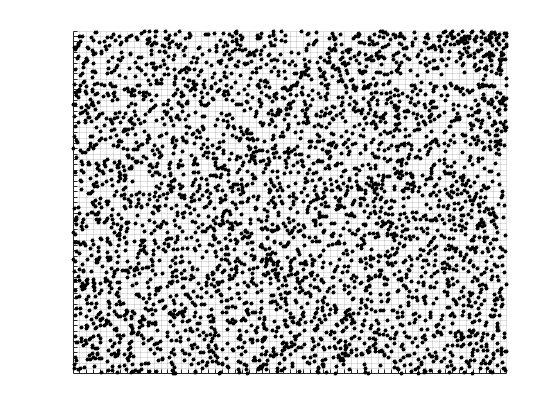
\includegraphics[width=\textwidth]{figures/psudo_init.png}
  \end{minipage} %
  \begin{minipage}[b]{0.49\textwidth}
    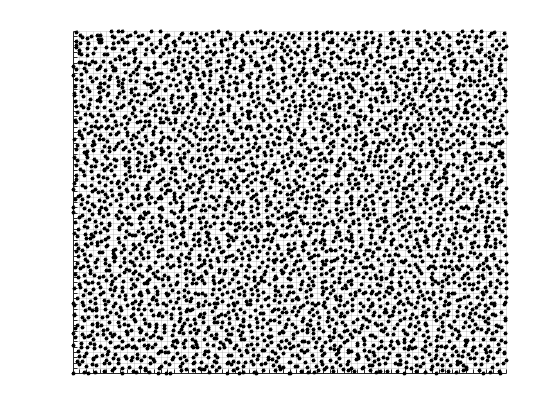
\includegraphics[width=\textwidth]{figures/uniform_init.png}

  \end{minipage}
  \caption[Uniform Particle Initialization]{Uniform Particle Initialization \textmd{(left) The generic random initialization of particle position \cite{mac_thesis}. (right) The uniform distribution of particle position by each cell \cite{mac_thesis}.}}
  \label{fig:part_init}
\end{figure}

The next step is to ``Move Particles". This algorithm consists of going through each particle and updating its position using its velocity and the chosen time-step. This is a purely decoupled event and therefore can be split into parallel operations, which has been implemented and is shown in Section \ref{sec:execution}. \par

The next step is to ``Perform Boundary Interactions". After moving a particle, it is checked to see if it exited its cell, and if so if it passed through a boundary on the way there. If so, the particle is processed through surface interactions. There are many types of surfaces that can be implemented in a DSMC simulation. A discussion of the ones implemented in this thesis are found in Section \ref{sec:models}. \par

The next step is to ``Insert New Particles". In this stage particles are introduced to the domain through Inlets specified by the user. New particles are randomly inserted in terms of position and velocity, but are inserted with the same distributions required in initialization. \par

The next step is to ``Sort Particles into Cells". Once the particles are all moved, all the new particles are added, the surface interactions are calculated, and the particles which are in new cells are linked back to those cells. This involves looking at nearby cells and determining within which cell the particle now lies, as well as removing particles no longer in the domain. \par

The next step is to ``Collide Particles". Now collisions are calculated between the particles. This involves using the sphere model for the particle and choosing collision partners through a selection method. A discussion on the models available in SINATRA can be found in Section \ref{sec:models}. These collisions will change the velocity of the particles. \par

The next step is to ``Sample Properties". Once this is completed, properties about the simulation can be sampled. Through sampling during the time-stepping loop, the analyst has the ability to view the simulation over time and determine if it has reached a steady state solution or view the transient or oscillatory nature of the fluid. This allows SINATRA to have the capacity to be a steady state or a transient simulation depending on the scenario and application. The method to sample properties in SINATRA can be found in Section \ref{sec:output}. \par

These steps continue until the simulation has completed the user specified time-steps. Then the simulation breaks from the loop, performs final data output, and ends the program. 




